\documentclass{article} % use larger type; default would be 10pt

\usepackage{pgfplots}
\usetikzlibrary{calc}
\usetikzlibrary{arrows}
\usetikzlibrary{patterns}
\usetikzlibrary{calc,intersections,through,backgrounds}
\usetikzlibrary{decorations.pathreplacing}
        \usepackage{xcolor} 
        \newcommand\degree[0]{^{\circ}}
        \newcommand\abs[1]{\left|#1\right|}
\usepackage{amsmath}
        \newcommand{\alert}[1]{\boldsymbol{\color{magenta}{#1}}}
        \newcommand{\blert}[1]{\boldsymbol{\color{blue}{#1}}}

\title{Play with TikZ}
\author{Just Us}
%\date{} % Activate to display a given date or no date (if empty),
         % otherwise the current date is printed 

\begin{document}
\maketitle

\section{Chap 4 Section 1}


fig-4-1-1

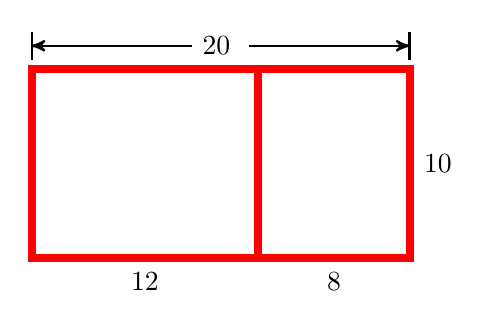
\begin{tikzpicture} [scale=1.2]
\draw[red, line width=1mm] (0,0) rectangle ++(4,2);
\draw[red, line width=1mm] (2.4,0) --++(0,2);
\draw[black,thick] (0,2.1)--++(0, 0.3);
\draw[black,thick] (4,2.1)--++(0, 0.3);
\draw[black,thick, <-, >=stealth'] (0,2.25)--++(1.7,0) node[right]{20};
\draw[black,thick, <-, >=stealth'] (4,2.25)--++(-1.7,0);
\node[below] at (1.2,-.05) {12};
\node[below] at (3.2,-.05) {8};
\node[right] at (4.05,1) {10};
\end{tikzpicture}
\newline


hp-4-1-29

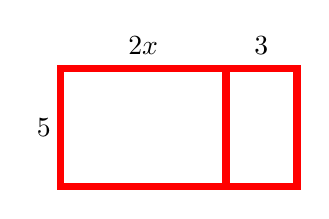
\begin{tikzpicture} 
\draw[red, line width=1mm] (0,0) rectangle ++(3,1.5);
\draw[red, line width=1mm] (2.1,0) --++(0,1.5);
\node[above] at (1.05,1.55) {$2x$};
\node[above] at (2.55,1.55) {$3$};
\node[left] at (0,0.75) {$5$};
\end{tikzpicture}
\newline


hp-4-1-29

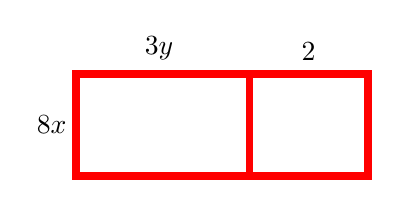
\begin{tikzpicture} 
\draw[red, line width=1mm] (0,0) rectangle ++(3.7,1.3);
\draw[red, line width=1mm] (2.2,0) --++(0,1.3);
\node[above] at (1.05,1.35) {$3y$};
\node[above] at (2.95,1.35) {$2$};
\node[left] at (0,0.65) {$8x$};
\end{tikzpicture}
\newline




\section{Chap 4 Section 2}


fig-4-2-ex3 

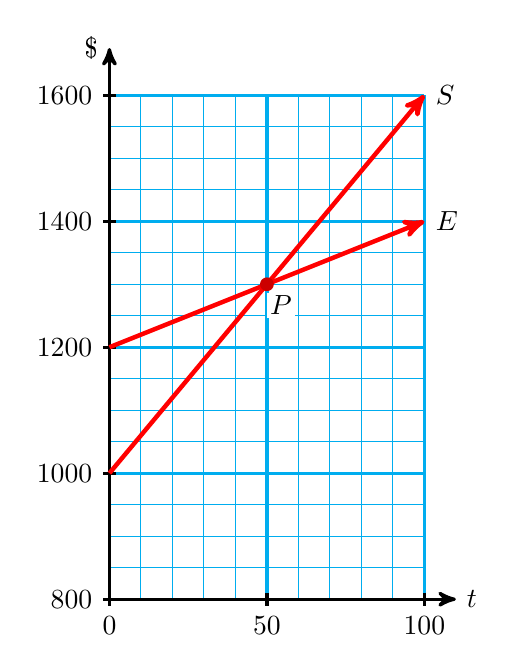
\begin{tikzpicture} [scale=.4]
\draw[cyan] (0,0) grid (10,16);
\foreach \x [evaluate=\x as \xi using int(10*\x)] in {0, 5,10} {
 \draw[cyan,very thick] (\x,0)--(\x,16);
 \draw[black,very thick] (\x, .2)--++(0,-.4) node[below]{$ \xi $};
 }
\foreach \x [evaluate=\x as \xi using int(50*\x+800)] in {0,4,8,12,16} {
 \draw[cyan,very thick] (0,\x)--(10,\x);
 \draw[black,very thick] (.2,\x)--++(-.4,0) node[left]{$ \xi $};
 }
\draw[black, very thick,->,>=stealth'] (0,0)--(11,0) node[right]{$t$};
\draw[black, very thick,->,>=stealth'] (0,0)--(0,17.5) node[left]{\$};
\draw[red, ultra thick, ->,>=stealth'] (0,4)--(10,16) node[right, text=black]{$ S $};
\draw[red, ultra thick, ->,>=stealth'] (0,8)--(10,12) node[right, text=black]{$ E $};
\filldraw[red!80!black] (5,10) circle (2mm) node[below right, yshift=-3, text=black, fill=white, inner sep=1] {$P$};
\end{tikzpicture}
\newline


fig-4-2-ex4

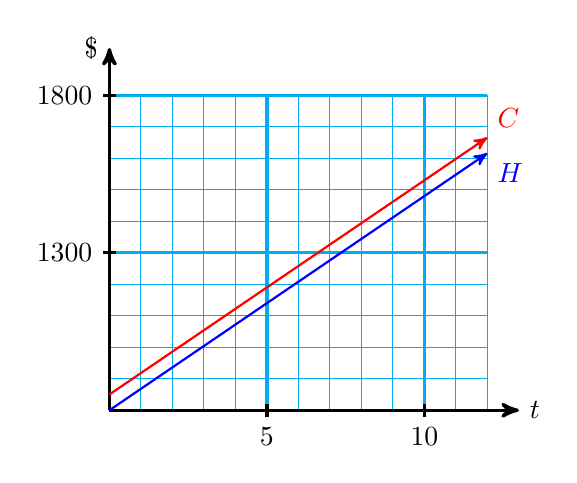
\begin{tikzpicture} [scale=.4]
\draw[cyan] (0,0) grid (12,10);
\foreach \x  in { 5,10} {
 \draw[cyan,very thick] (\x,0)--(\x,10);
 \draw[black,very thick] (\x, .2)--++(0,-.4) node[below]{$ \x $};
 }
\foreach \x [evaluate=\x as \xi using int(100*\x+800)] in {5,10} {
 \draw[cyan,very thick] (0,\x)--(12,\x);
 \draw[black,very thick] (.2,\x)--++(-.4,0) node[left]{$ \xi $};
 }
\draw[black, very thick,->,>=stealth'] (0,0)--(13,0) node[right]{$t$};
\draw[black, very thick,->,>=stealth'] (0,0)--(0,11.5) node[left]{\$};
\draw[red, thick, ->,>=stealth'] (0,.5)--(12,{(50+68*12)/100}) node[above right]{$ C $};
\draw[blue, thick, ->,>=stealth'] (0,0)--(12,{68*12/100}) node[below right]{$ H $};
\end{tikzpicture}
\newline


fig-4-2-ex5

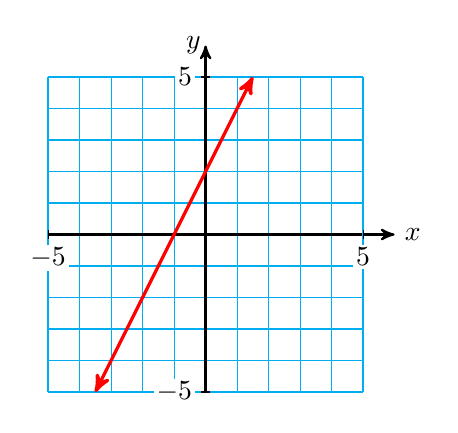
\begin{tikzpicture} [scale=.4]
\draw[cyan] (-5,-5) grid (5,5);
\draw[black, thick, ->, >=stealth'] (-5,0)--(6,0) node[right]{$x$};
\draw[black, thick, ->, >=stealth'] (0,-5)--(0,6) node[left, xshift=2]{$y$};
\foreach \x  in  {-5, 5} {
 \draw[cyan, thick] (\x,-5) --++(0,10);
 \draw[cyan, thick] (-5,\x) --++(10,0);
 \draw[black] (\x,.15) --++(0,-.3) node[below, yshift=-2, fill=white, inner sep=1]   {$\x$};
 \draw[black] (.15,\x) --++(-.3,0) node[left, xshift=-2, fill=white, inner sep=1]   {$\x$};
}
\draw[red, very thick,<->, >=stealth'] (-3.5,-5)--(3/2,5);
\end{tikzpicture}
\newline


fig-4-2-1

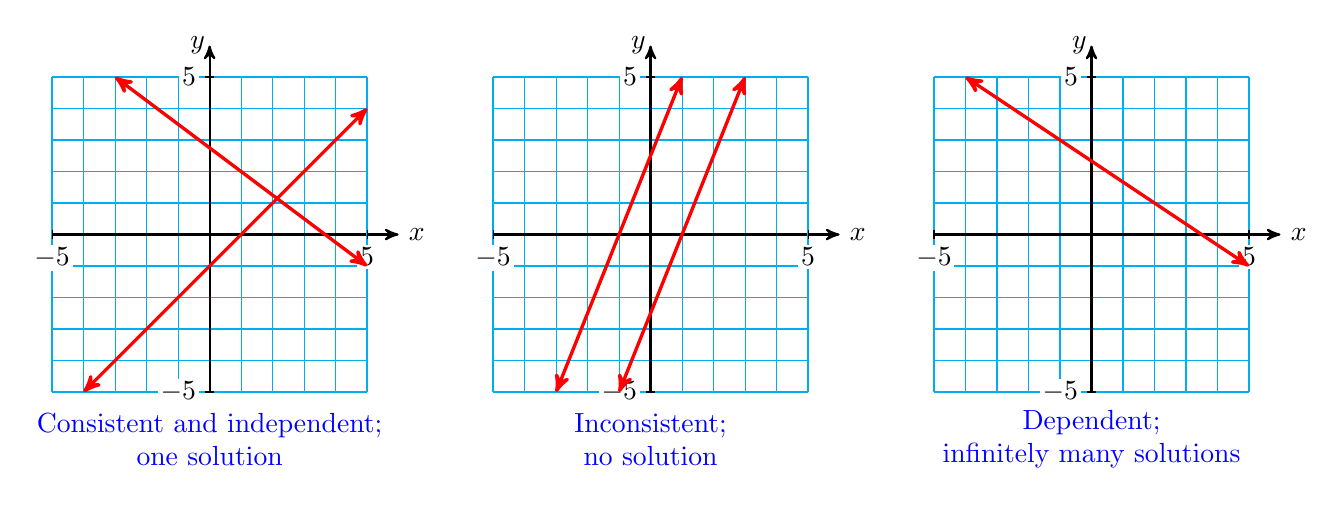
\begin{tikzpicture} [scale=.4]
\draw[cyan] (-5,-5) grid (5,5);
\draw[black, thick, ->, >=stealth'] (-5,0)--(6,0) node[right]{$x$};
\draw[black, thick, ->, >=stealth'] (0,-5)--(0,6) node[left, xshift=2]{$y$};
\foreach \x  in  {-5, 5} {
 \draw[cyan, thick] (\x,-5) --++(0,10);
 \draw[cyan, thick] (-5,\x) --++(10,0);
 \draw[black] (\x,.15) --++(0,-.3) node[below, yshift=-2, fill=white, inner sep=1]   {$\x$};
 \draw[black] (.15,\x) --++(-.3,0) node[left, xshift=-2, fill=white, inner sep=1]   {$\x$};
}
\draw[red, very thick,<->, >=stealth'] (-4,-5)--(5,4);
\draw[red, very thick,<->, >=stealth'] (-3,5)--(5,-1);
\node[text=blue, align=center] at (0,-6.5) {Consistent and independent;\\one solution};

\def\delx{14};
\draw[cyan] ({\delx-5},-5) grid ({\delx+5},5);
\draw[black, thick, ->, >=stealth'] ({\delx-5},0)--({\delx+6},0) node[right]{$x$};
\draw[black, thick, ->, >=stealth'] (\delx,-5)--++(0,11) node[left, xshift=2]{$y$};
\foreach \x  in  {-5, 5} {
 \draw[cyan, thick] ({\delx+\x},-5) --++(0,10);
 \draw[cyan, thick] ({\delx-5},\x) --++(10,0);
 \draw[black] ({\delx+\x},.15) --++(0,-.3) node[below, yshift=-2, fill=white, inner sep=1]   {$\x$};
 \draw[black] ({\delx+.15},\x) --++(-.3,0) node[left, xshift=-2, fill=white, inner sep=1]   {$\x$};
}
\draw[red, very thick,<->, >=stealth'] ({\delx-3},-5)--({\delx+1},5);
\draw[red, very thick,<->, >=stealth'] ({\delx-1},-5)--({\delx+3},5);
\node[text=blue, align=center] at (\delx,-6.5) {Inconsistent;\\no solution};

\def\delx{28};
\draw[cyan] ({\delx-5},-5) grid ({\delx+5},5);
\draw[black, thick, ->, >=stealth'] ({\delx-5},0)--({\delx+6},0) node[right]{$x$};
\draw[black, thick, ->, >=stealth'] (\delx,-5)--++(0,11) node[left, xshift=2]{$y$};
\foreach \x  in  {-5, 5} {
 \draw[cyan, thick] ({\delx+\x},-5) --++(0,10);
 \draw[cyan, thick] ({\delx-5},\x) --++(10,0);
 \draw[black] ({\delx+\x},.15) --++(0,-.3) node[below, yshift=-2, fill=white, inner sep=1]   {$\x$};
 \draw[black] ({\delx+.15},\x) --++(-.3,0) node[left, xshift=-2, fill=white, inner sep=1]   {$\x$};
}
\draw[red, very thick,<->, >=stealth'] ({\delx-4},5)--({\delx+5},-1);
\node[text=blue, align=center] at (\delx,-6.5) {Dependent;\\infinitely many solutions};
\end{tikzpicture}
\newline

fig-4-2-ex6

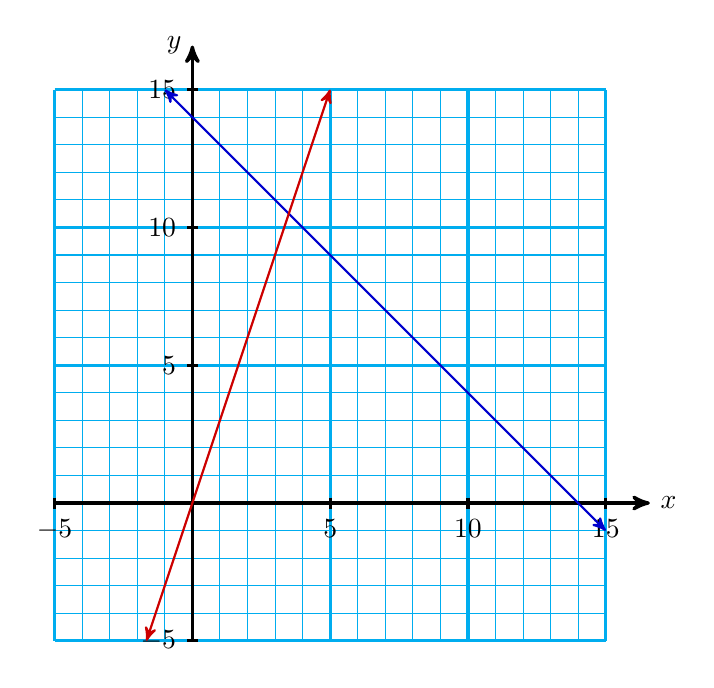
\begin{tikzpicture} [scale=.35]
\draw[cyan] (-5,-5) grid (15,15);
\foreach \x  in { -5, 5,10,15} {
 \draw[cyan,very thick] (\x,-5)--(\x,15);
 \draw[black,very thick] (\x, .2)--++(0,-.4) node[below]{$ \x $};
 \draw[cyan,very thick] (-5,\x)--(15,\x);
 \draw[black,very thick] (.2,\x)--++(-.4,0) node[left]{$ \x $};
 }
\draw[black, very thick,->,>=stealth'] (-5,0)--(16.6,0) node[right]{$x$};
\draw[black, very thick,->,>=stealth'] (0,-5)--(0,16.6) node[left]{$y$};
\draw[blue!80!black, thick, <->,>=stealth'] (-1,15)--(15,-1);
\draw[red!80!black, thick, <->,>=stealth'] (-5/3,-5)--(5,15);
\end{tikzpicture}
\newline


hp-4-2-13

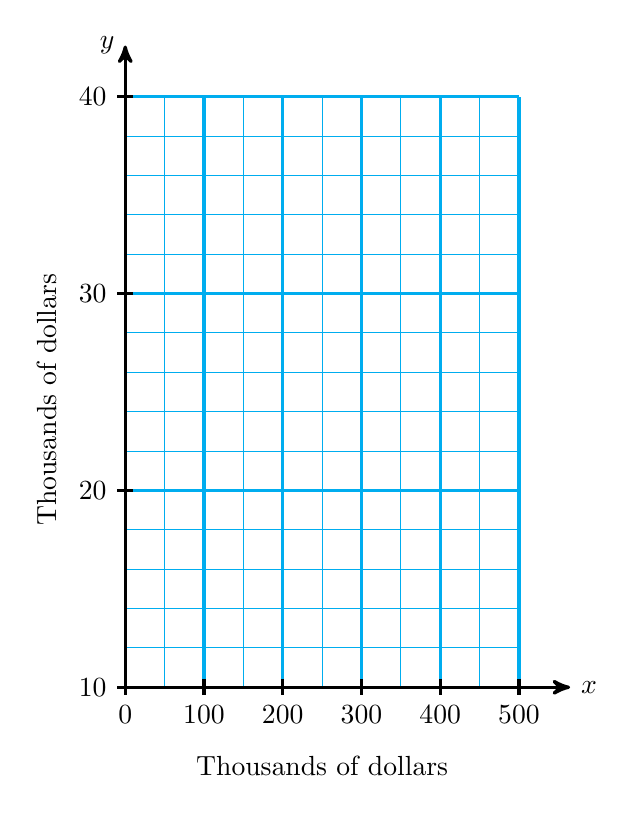
\begin{tikzpicture} [scale=.5]
\draw[cyan] (0,0) grid (10,15);
\foreach \x [evaluate=\x as \xi using int(50*\x)] in {0, 2,4,6,8,10} {
 \draw[cyan,very thick] (\x,0)--(\x,15);
 \draw[black,very thick] (\x, .2)--++(0,-.4) node[below]{$ \xi $};
 }
\foreach \x [evaluate=\x as \xi using int(2*\x+10)] in {0, 5,10,15} {
 \draw[cyan,very thick] (0,\x)--(10,\x);
 \draw[black,very thick] (.2,\x)--++(-.4,0) node[left]{$ \xi $};
 }
\draw[black, very thick,->,>=stealth'] (0,0)--(11.3,0) node[right]{$x$};
\draw[black, very thick,->,>=stealth'] (0,0)--(0,16.3) node[left]{$y$};
\node[below] at (5,-1.5) {Thousands of dollars};
\node[label=below:\rotatebox{90}{Thousands of dollars}] at (-2,11) {};
\end{tikzpicture}
\newline


hp-4-2-14

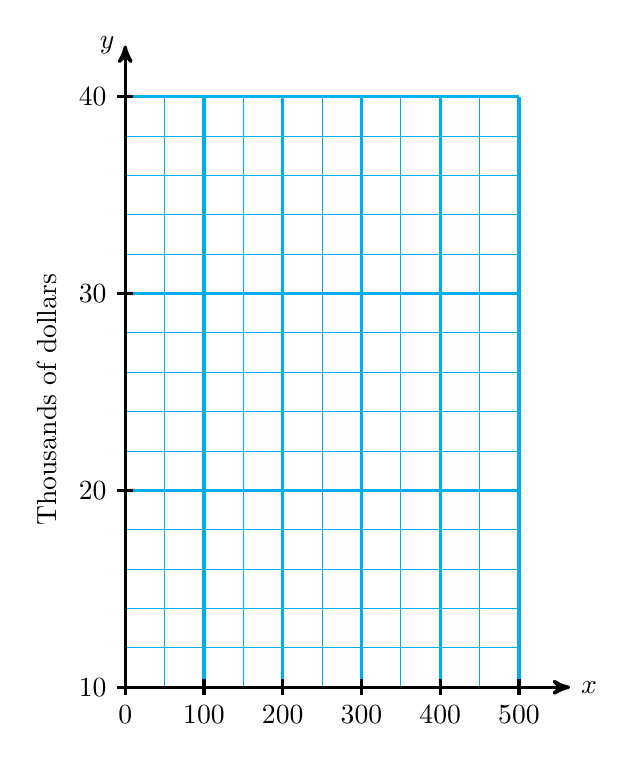
\begin{tikzpicture} [scale=.5]
\draw[cyan] (0,0) grid (10,15);
\foreach \x [evaluate=\x as \xi using int(50*\x)] in {0, 2,4,6,8,10} {
 \draw[cyan,very thick] (\x,0)--(\x,15);
 \draw[black,very thick] (\x, .2)--++(0,-.4) node[below]{$ \xi $};
 }
\foreach \x [evaluate=\x as \xi using int(2*\x+10)] in {0, 5,10,15} {
 \draw[cyan,very thick] (0,\x)--(10,\x);
 \draw[black,very thick] (.2,\x)--++(-.4,0) node[left]{$ \xi $};
 }
\draw[black, very thick,->,>=stealth'] (0,0)--(11.3,0) node[right]{$x$};
\draw[black, very thick,->,>=stealth'] (0,0)--(0,16.3) node[left]{$y$};
\node[label=below:\rotatebox{90}{Thousands of dollars}] at (-2,11) {};
\end{tikzpicture}
\newline


hp-4-2-15

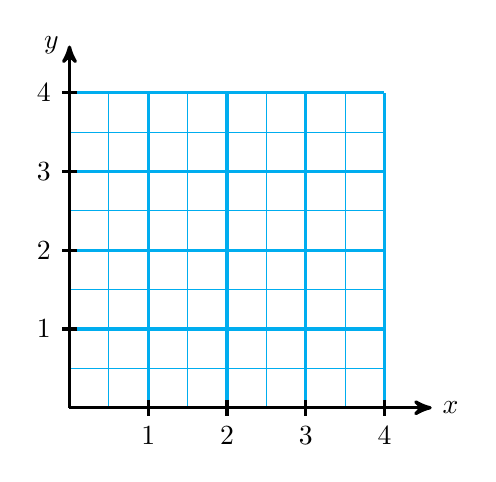
\begin{tikzpicture} [scale=1]
\draw[cyan] (0,0) grid[step=1/2] (4,4);
\foreach \x  in {1,2,3,4} {
 \draw[cyan,very thick] (\x,0)--(\x,4);
 \draw[black,very thick] (\x, .1)--++(0,-.2) node[below]{$ \x $};
 \draw[cyan,very thick] (0,\x)--(4,\x);
 \draw[black,very thick] (.1,\x)--++(-.2,0) node[left]{$ \x $};
 }
\draw[black, very thick,->,>=stealth'] (0,0)--(4.6,0) node[right]{$x$};
\draw[black, very thick,->,>=stealth'] (0,0)--(0,4.6) node[left]{$y$};
\end{tikzpicture}
\newline


hp-4-2-16

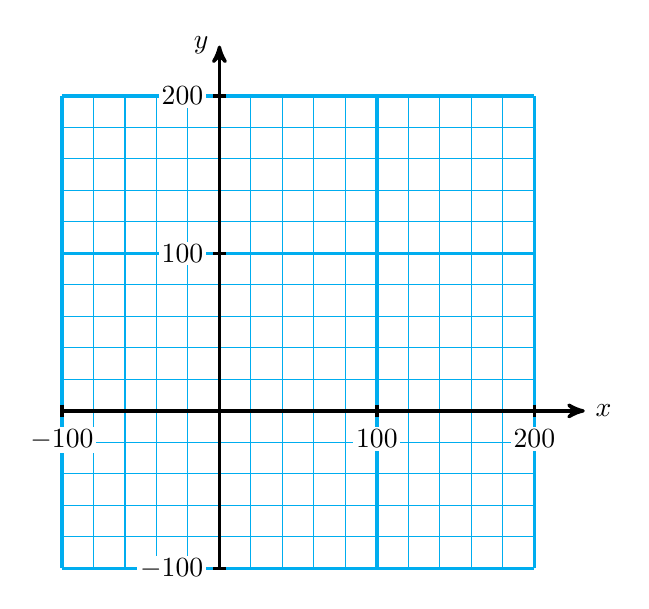
\begin{tikzpicture} [scale=.4]
\draw[cyan] (-5,-5) grid (10,10);
\foreach \x [evaluate=\x as \xi using int(20*\x)]in {-5,5,10} {
 \draw[cyan,very thick] (\x,-5)--(\x,10);
 \draw[black,very thick] (\x, .2)--++(0,-.4) node[below, yshift=-3, fill=white, inner sep=1]{$ \xi $};
 \draw[cyan,very thick] (-5,\x)--(10,\x);
 \draw[black,very thick] (.2,\x)--++(-.4,0) node[left,xshift=-2, fill=white, inner sep=1]{$ \xi $};
 }
\draw[black, very thick,->,>=stealth'] (-5,0)--(11.6,0) node[right]{$x$};
\draw[black, very thick,->,>=stealth'] (0,-5)--(0,11.6) node[left]{$y$};
\end{tikzpicture}
\newline

\section{Chap 4 Section 3}

fig-4-2-ex3 from 4.2 Example 3
\newline

fig-4-3-1

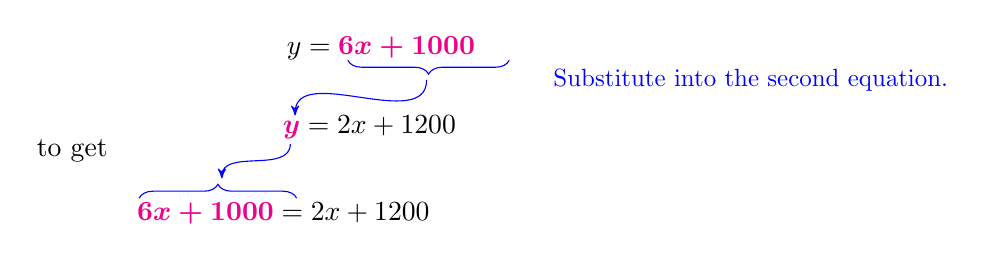
\begin{tikzpicture}
\node[right] at (0,0) {$y=\alert{6x+1000}$};
\coordinate (A) at (2.95,-.15);
\draw [blue,decorate,decoration={brace,amplitude=5pt}] (A) -- ++(-2.05,0) node [below right,xshift=2.5cm, scale=.9] {Substitute into the second equation.};
\coordinate (B) at (-.05,-1.);
\node[right] at (B) {$\alert{y}=2x+1200$};
\draw[blue,->,>=stealth'] (1.9,-.4) to [out=270,in=90] ($(B)+(.28,.15)$);
\coordinate (C) at (-1.9,-2.1);
\node[right] at (C) {$\alert{6x+1000}=2x+1200$};
\draw [blue,decorate,decoration={brace,amplitude=5pt}] (C)++(.15,.2) -- ++(2,0);
\draw[blue,->,>=stealth'] (B)++(.22,-.21) to [out=270,in=90] ($(C)+(1.2,0.45)$);
\node at ($(C)+(-.7,.8)$) {to get};
\end{tikzpicture}
\newline


fig-4-3-ex2

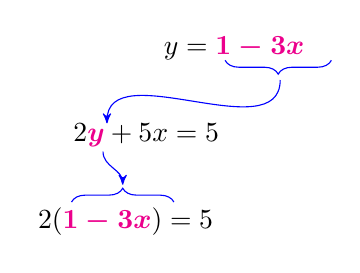
\begin{tikzpicture}
\node[right] at (0,0) {$y=\alert{1-3x}$};
\coordinate (A) at (2.25,-.15);
\draw [blue,decorate,decoration={brace,amplitude=5pt}] (A) -- ++(-1.35,0);
\coordinate (B) at (-1.15,-1.1);
\node[right] at (B) {$2\alert{y}+5x=5$};
\draw[blue,->,>=stealth'] (1.6,-.4) to [out=270,in=90] ($(B)+(0.55,.15)$);
\coordinate (C) at (-1.6,-2.2);
\node[right] at (C) {$2(\alert{1-3x})=5$};
\draw [blue,decorate,decoration={brace,amplitude=5pt}] (C)++(.55,.25) -- ++(1.3,0);
\draw[blue,->,>=stealth'] (B)++(.5,-.21) to [out=270,in=90] ($(C)+(1.2,0.47)$);
\end{tikzpicture}
\newline

fig-4-3-ex6a

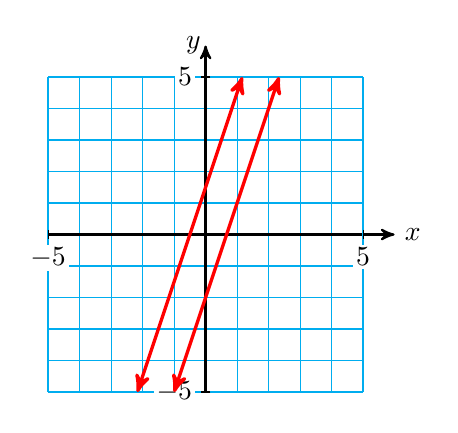
\begin{tikzpicture}[scale=.4]
\def\delx{0};
\draw[cyan] ({-5},-5) grid ({5},5);
\draw[black, thick, ->, >=stealth'] (-5,0)--(6,0) node[right]{$x$};
\draw[black, thick, ->, >=stealth'] (0,-5)--++(0,11) node[left, xshift=2]{$y$};
\foreach \x  in  {-5, 5} {
 \draw[cyan, thick] ({\x},-5) --++(0,10);
 \draw[cyan, thick] ({-5},\x) --++(10,0);
 \draw[black] ({\x},.15) --++(0,-.3) node[below, yshift=-2, fill=white, inner sep=1]   {$\x$};
 \draw[black] ({.15},\x) --++(-.3,0) node[left, xshift=-2, fill=white, inner sep=1]   {$\x$};
}
\draw[red, very thick,<->, >=stealth'] (-1,-5)--(7/3,5);
\draw[red, very thick,<->, >=stealth'] (-13/6,-5)--(7/6,5);
\end{tikzpicture}
\newline

fig-4-3-ex6b
\newline

\section{Chap 4 Section 4}

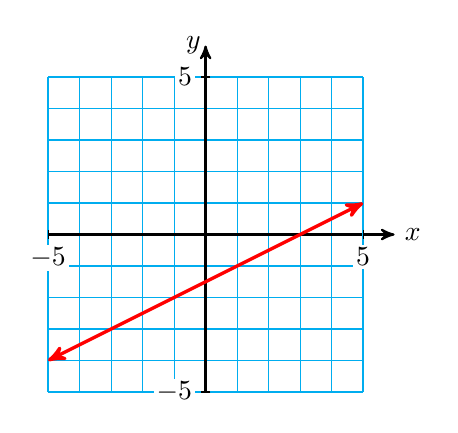
\begin{tikzpicture}[scale=.4]
\def\delx{0};
\draw[cyan] (-5,-5) grid (5,5);
\draw[black, thick, ->, >=stealth'] (-5,0)--(6,0) node[right]{$x$};
\draw[black, thick, ->, >=stealth'] (0,-5)--++(0,11) node[left, xshift=2]{$y$};
\foreach \x  in  {-5, 5} {
 \draw[cyan, thick] ({\x},-5) --++(0,10);
 \draw[cyan, thick] ({-5},\x) --++(10,0);
 \draw[black] ({\x},.15) --++(0,-.3) node[below, yshift=-2, fill=white, inner sep=1]   {$\x$};
 \draw[black] ({.15},\x) --++(-.3,0) node[left, xshift=-2, fill=white, inner sep=1]   {$\x$};
}
\draw[red, very thick,<->, >=stealth'] (-5,-4)--(5,1);
\end{tikzpicture}
\newline


hp-4-4-9ans

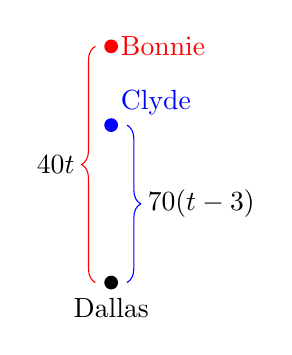
\begin{tikzpicture} 
\coordinate (O) at (0,0);
\coordinate (B) at (0,3);
\coordinate (C) at (0,2);
\filldraw[black] (O) circle (.8mm) node[below, yshift=-2] {Dallas};
\filldraw[red] (B) circle (.8mm) node[right] {Bonnie};
\filldraw[blue] (C) circle (.8mm) node[above right] {Clyde};
\draw [red,decorate,decoration={brace,amplitude=5pt}] (O)++(-.2,0) -- ($(B)+(-.2,0)$) node [black, left, xshift=-4,midway] {$40t$};
\draw [blue,decorate,decoration={brace,amplitude=5pt}] (C)++(.2,0) -- ($(O)+(.2,0)$) node [black, right, xshift=4,midway] {$70(t-3)$};

\end{tikzpicture}
\newline


hp-4-4-12

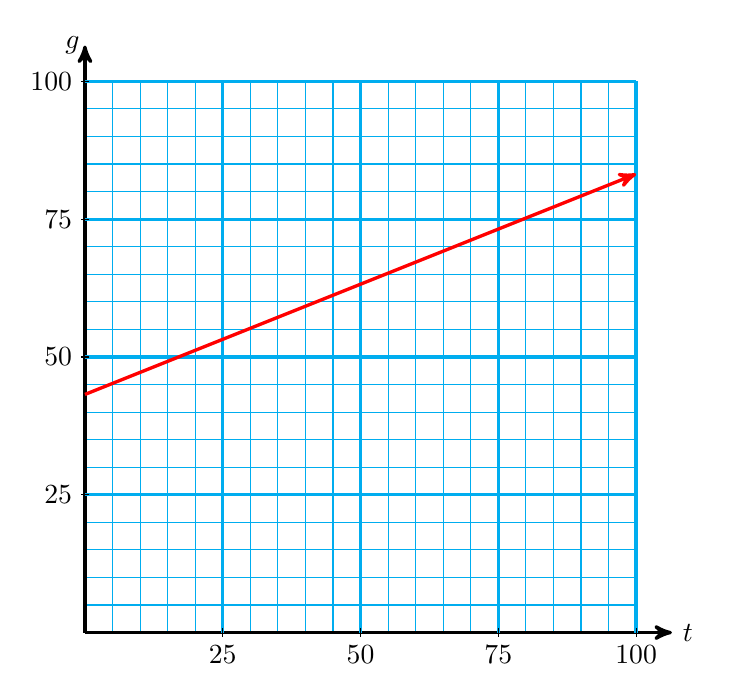
\begin{tikzpicture} [scale=.35]
\draw[cyan] (0,0) grid (20,20);
\draw[black,very thick, ->, >=stealth'] (0,0)--(21.3,0) node[right]{$t$};
\draw[black,very thick, ->, >=stealth'] (0,0)--(0,21.3) node[left, xshift=2]{$g$};
\foreach \x [evaluate=\x as \xi using int(5*\x)] in  {5,10,15,20} {
 \draw[cyan, very thick] (\x,0) --++(0,20);
 \draw[cyan, very thick] (0,\x) --++(20,0);
 \draw[black] (\x,.15) --++(0,-.3) node[below, yshift=-2, fill=white, inner sep=1]   {$\xi$};
 \draw[black] (.15,\x) --++(-.3,0) node[left, xshift=-2, fill=white, inner sep=1]   {$\xi$};
}
\draw[red, very thick, ->, >=stealth'] (0,{.6*72/5})--(20,{(.6*72 +.4*100)/5});
\end{tikzpicture}
\newline

\section{Chap 4 Section 5}


fig-4-5-ex1

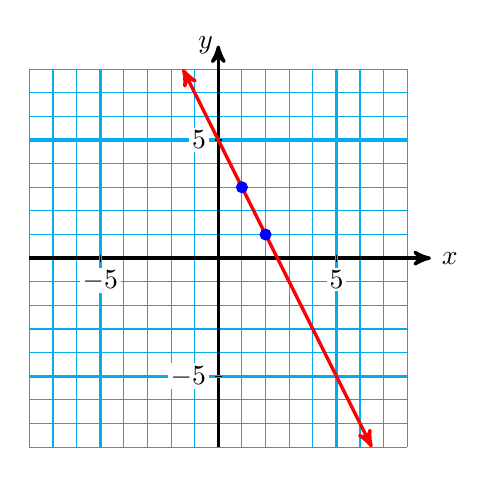
\begin{tikzpicture} [scale=.3]
\draw[cyan] (-8,-8) grid (8,8);
\draw[black,very thick, ->, >=stealth'] (-8,0)--(9,0) node[right]{$x$};
\draw[black,very thick, ->, >=stealth'] (0,-8)--(0,9) node[left, xshift=2]{$y$};
\foreach \x  in  {-5, 5} {
 \draw[cyan, very thick] (\x,-8) --++(0,16);
 \draw[cyan, very thick] (-8,\x) --++(16,0);
 \draw[black] (\x,.15) --++(0,-.3) node[below, yshift=-2, fill=white, inner sep=1]   {$\x$};
 \draw[black] (.15,\x) --++(-.3,0) node[left, xshift=-2, fill=white, inner sep=1]   {$\x$};
}
\draw[red, very thick, <->, >=stealth'] (-3/2,8)--(13/2,-8);
\filldraw[blue] (1,3) circle (2.3mm);
\filldraw[blue] (2,1) circle (2.3mm);
\end{tikzpicture}
\newline


fig-4-5-ex2

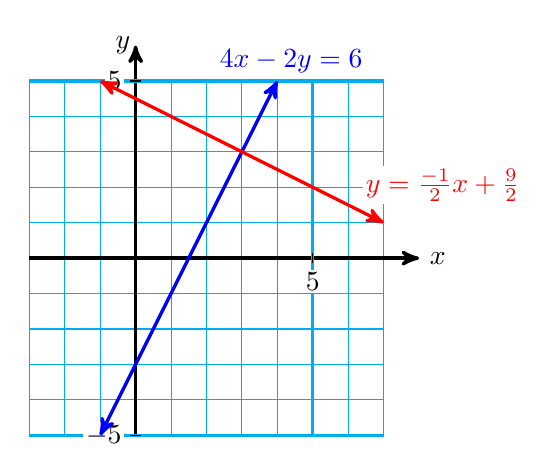
\begin{tikzpicture} [scale=.45]
\draw[cyan] (-3,-5) grid (7,5);
\draw[black,very thick, ->, >=stealth'] (-3,0)--(8,0) node[right]{$x$};
\draw[black,very thick, ->, >=stealth'] (0,-5)--(0,6) node[left, xshift=2]{$y$};
\foreach \x  in  {-5, 5} {
 \draw[cyan, very thick] (-3,\x) --++(10,0);
 \draw[black] (.15,\x) --++(-.3,0) node[left, xshift=-2, fill=white, inner sep=1]   {$\x$};
}
 \draw[cyan, very thick] (5,-5) --(5,5);
 \draw[black] (5,.15) --++(0,-.3) node[below, yshift=-2, fill=white, inner sep=1]   {$5$};
\draw[blue, very thick, <->, >=stealth'] (-1,-5)--(4,5) node[above, xshift=5, yshift=-1] {$4x-2y=6$};
\draw[red, very thick, <->, >=stealth'] (-1,5)--(7,1) node[above right, xshift=-8, yshift=6, fill=white, inner sep=1] {$y=\frac{-1}{2}x+\frac{9}2{•}$};
\end{tikzpicture}
\newline

fig-4-5-ex3

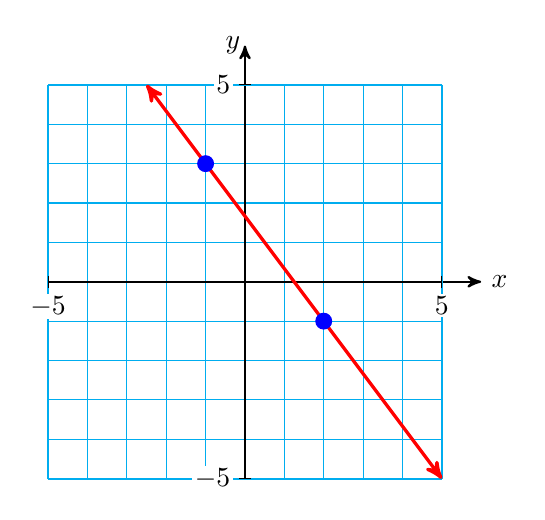
\begin{tikzpicture}[scale=.5]
\draw[cyan] (-5,-5) grid (5,5);
\draw[black, thick, ->, >=stealth'] (-5,0)--(6,0) node[right]{$x$};
\draw[black, thick, ->, >=stealth'] (0,-5)--++(0,11) node[left, xshift=2]{$y$};
\foreach \x  in  {-5, 5} {
 \draw[cyan, thick] ({\x},-5) --++(0,10);
 \draw[cyan, thick] ({-5},\x) --++(10,0);
 \draw[black] ({\x},.15) --++(0,-.3) node[below, yshift=-2, fill=white, inner sep=1]   {$\x$};
 \draw[black] ({.15},\x) --++(-.3,0) node[left, xshift=-2, fill=white, inner sep=1]   {$\x$};
}
\draw[red, very thick,<->, >=stealth'] (-5/2,5)--(5,-5);
\filldraw[blue] (2,-1) circle (2.mm);
\filldraw[blue] (-1,3) circle (2.mm);
\end{tikzpicture}
\newline

hp-4-5-1ans

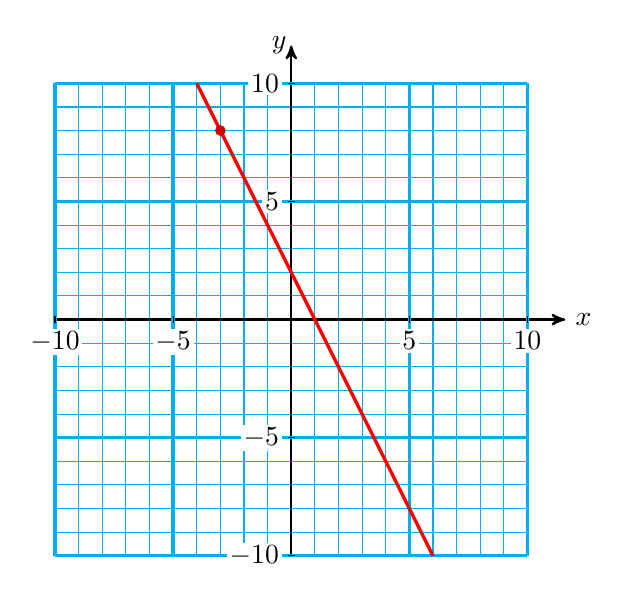
\begin{tikzpicture} [scale=.3]
\coordinate (O) at (0,0);
\draw[cyan] (-10,-10) grid (10,10);
\draw[black,thick, ->, >=stealth'] (-10,0)--(11.6,0) node[right]{$x$};
\draw[black,thick, ->, >=stealth'] (0,-10)--(0,11.6) node[left, xshift=2]{$y$};
\foreach \x in  {-5, 5, -10, 10} {
 \draw[cyan, very thick] (\x,-10) --++(0,20);
 \draw[cyan, very thick] (-10,\x) --++(20,0);
 \draw[black] (\x,.15) --++(0,-.3)  node[below, yshift=-2, fill=white, inner sep=1]   {$\x$};
 \draw[black] (.15,\x) --++(-.3,0)  node[left, xshift=-2, fill=white, inner sep=1]   {$\x$};
}
\draw[red,very thick] (-4,10)--(6,-10);
\filldraw[red!80!black] (-3,8) circle (2mm);
\end{tikzpicture}
\newline\newline

hp-4-5-3ans

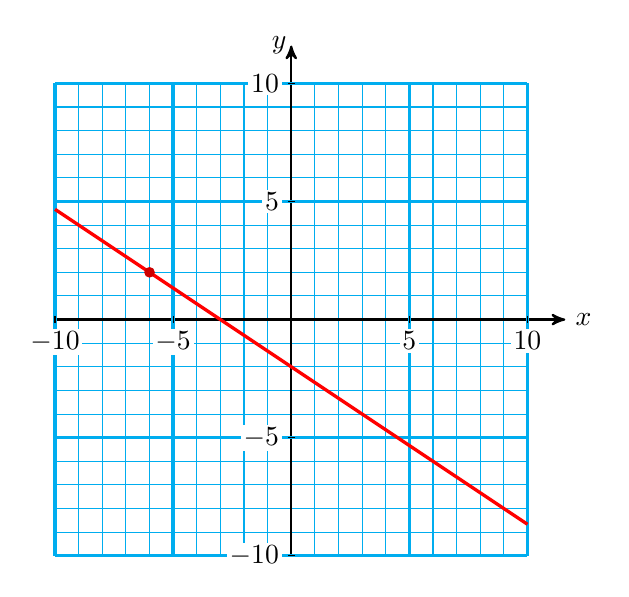
\begin{tikzpicture} [scale=.3]
\coordinate (O) at (0,0);
\draw[cyan] (-10,-10) grid (10,10);
\draw[black,thick, ->, >=stealth'] (-10,0)--(11.6,0) node[right]{$x$};
\draw[black,thick, ->, >=stealth'] (0,-10)--(0,11.6) node[left, xshift=2]{$y$};
\foreach \x in  {-5, 5, -10, 10} {
 \draw[cyan, very thick] (\x,-10) --++(0,20);
 \draw[cyan, very thick] (-10,\x) --++(20,0);
 \draw[black] (\x,.15) --++(0,-.3)  node[below, yshift=-2, fill=white, inner sep=1]   {$\x$};
 \draw[black] (.15,\x) --++(-.3,0)  node[left, xshift=-2, fill=white, inner sep=1]   {$\x$};
}
\draw[red,very thick] (-10,14/3)--(10,-26/3);
\filldraw[red!80!black] (-6,2) circle (2mm);
\end{tikzpicture}
\newline\newline

hp-4-5-5ans

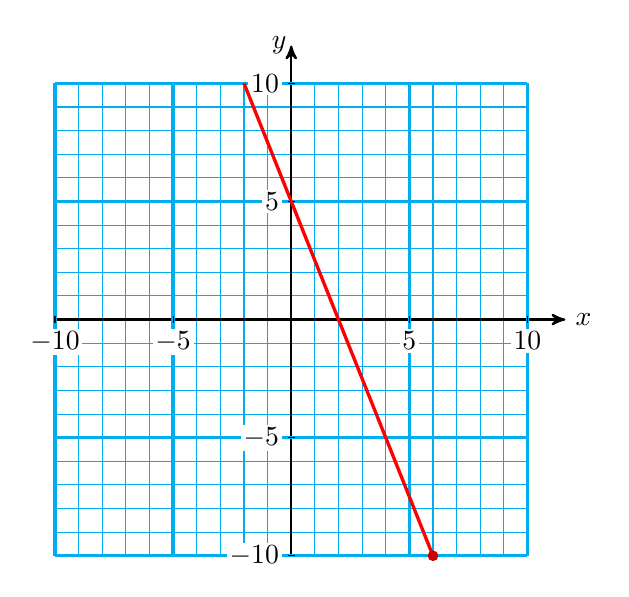
\begin{tikzpicture} [scale=.3]
\coordinate (O) at (0,0);
\draw[cyan] (-10,-10) grid (10,10);
\draw[black,thick, ->, >=stealth'] (-10,0)--(11.6,0) node[right]{$x$};
\draw[black,thick, ->, >=stealth'] (0,-10)--(0,11.6) node[left, xshift=2]{$y$};
\foreach \x in  {-5, 5, -10, 10} {
 \draw[cyan, very thick] (\x,-10) --++(0,20);
 \draw[cyan, very thick] (-10,\x) --++(20,0);
 \draw[black] (\x,.15) --++(0,-.3)  node[below, yshift=-2, fill=white, inner sep=1]   {$\x$};
 \draw[black] (.15,\x) --++(-.3,0)  node[left, xshift=-2, fill=white, inner sep=1]   {$\x$};
}
\draw[red,very thick] (6,-10)--(-2,10);
\filldraw[red!80!black] (6,-10) circle (2mm);
\end{tikzpicture}
\newline\newline


hp-4-5-13

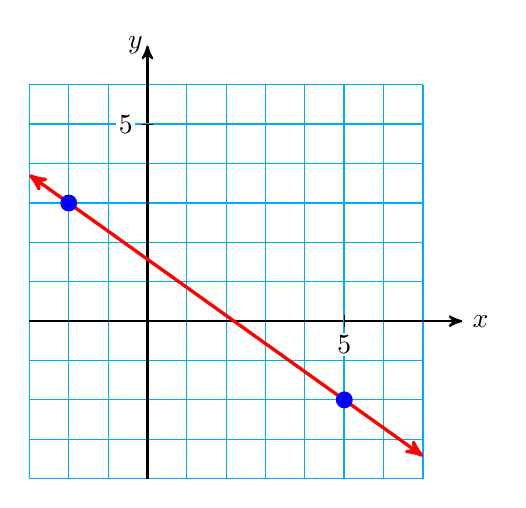
\begin{tikzpicture}[scale=.5]
\draw[cyan] (-3,-4) grid (7,6);
\draw[black, thick, ->, >=stealth'] (-3,0)--++(11,0) node[right]{$x$};
\draw[black, thick, ->, >=stealth'] (0,-4)--++(0,11) node[left, xshift=2]{$y$};
\foreach \x  in  { 5} {
 \draw[cyan, thick] ({\x},-4) --++(0,10);
 \draw[cyan, thick] (-3,\x) --++(10,0);
 \draw[black] ({\x},.15) --++(0,-.3) node[below, yshift=-2, fill=white, inner sep=1]   {$\x$};
 \draw[black] ({.15},\x) --++(-.3,0) node[left, xshift=-2, fill=white, inner sep=1]   {$\x$};
}
\draw[red, very thick,<->, >=stealth'] (-3,26/7)--(7,-24/7);
\filldraw[blue] (-2,3) circle (2.mm);
\filldraw[blue] (5,-2) circle (2.mm);
\end{tikzpicture}
\newline

hp-4-5-14

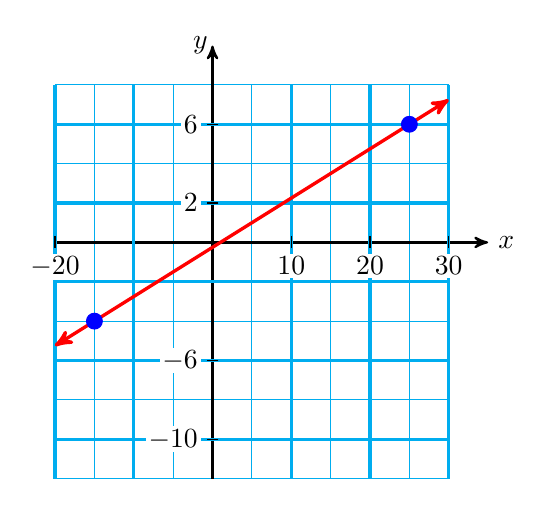
\begin{tikzpicture}[scale=.5]
\draw[cyan] (-4,-6) grid (6,4);
\draw[black, thick, ->, >=stealth'] (-4,0)--++(11,0) node[right]{$x$};
\draw[black, thick, ->, >=stealth'] (0,-6)--++(0,11) node[left, xshift=2]{$y$};
\draw[cyan, very thick] (-2,-6) --++(0,10);
\draw[cyan, very thick] (-4,-1) --++(10,0);
\foreach \x [evaluate=\x as \xi using int(5*\x)] in  {-4,2,4,6 } {
 \draw[cyan, very thick] (\x,-6) --++(0,10);
 \draw[black] ({\x},.15) --++(0,-.3) node[below, yshift=-2, fill=white, inner sep=1]   {$\xi$};
}
\foreach \x [evaluate=\x as \xi using int(2*\x)] in  {-5,-3, 1,3 } {
 \draw[cyan, very thick] (-4,\x) --++(10,0);
 \draw[black] ({.15},\x) --++(-.3,0) node[left, xshift=-2, fill=white, inner sep=1]   {$\xi$};
}
\draw[red, very thick,<->, >=stealth'] (-4,-21/8)--(6,29/8);
\filldraw[blue] (-3,-2) circle (2.mm);
\filldraw[blue] (5,3) circle (2.mm);
\end{tikzpicture}
\newline

hp-4-5-15

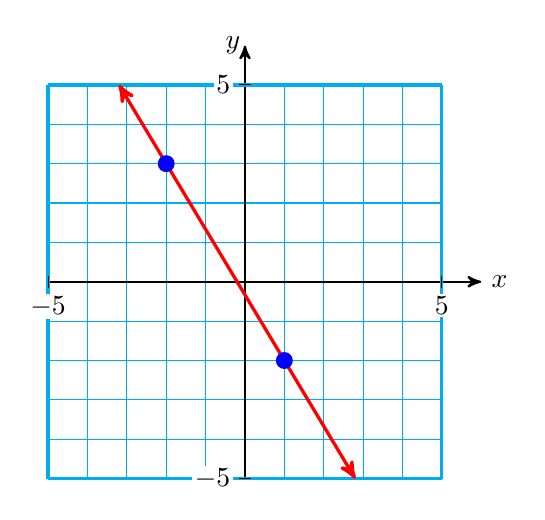
\begin{tikzpicture}[scale=.5]
\draw[cyan] (-5,-5) grid (5,5);
\draw[black, thick, ->, >=stealth'] (-5,0)--++(11,0) node[right]{$x$};
\draw[black, thick, ->, >=stealth'] (0,-5)--++(0,11) node[left, xshift=2]{$y$};
\foreach \x  in  {-5,5} {
 \draw[cyan, very thick] (\x,-5) --++(0,10);
 \draw[black] ({\x},.15) --++(0,-.3) node[below, yshift=-2, fill=white, inner sep=1]   {$\x$};
 \draw[cyan, very thick] (-5,\x) --++(10,0);
 \draw[black] ({.15},\x) --++(-.3,0) node[left, xshift=-2, fill=white, inner sep=1]   {$\x$};
}
\draw[red, very thick,<->, >=stealth'] (-16/5,5)--(14/5,-5);
\filldraw[blue] (-2,3) circle (2.mm);
\filldraw[blue] (1,-2) circle (2.mm);
\end{tikzpicture}
\newline

hp-4-5-16

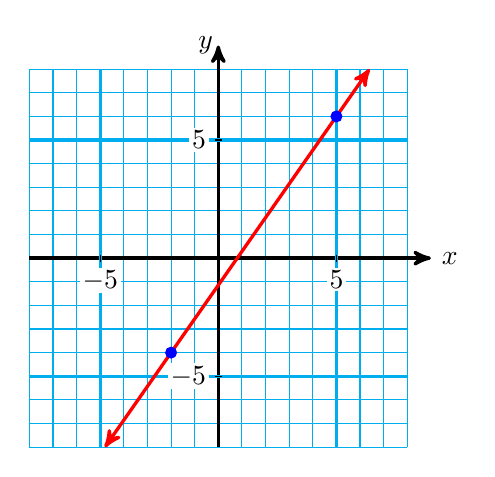
\begin{tikzpicture}[scale=.3]
\draw[cyan] (-8,-8) grid (8,8);
\draw[black,very thick, ->, >=stealth'] (-8,0)--(9,0) node[right]{$x$};
\draw[black,very thick, ->, >=stealth'] (0,-8)--(0,9) node[left, xshift=2]{$y$};
\foreach \x  in  {-5, 5} {
 \draw[cyan, very thick] (\x,-8) --++(0,16);
 \draw[cyan, very thick] (-8,\x) --++(16,0);
 \draw[black] (\x,.15) --++(0,-.3) node[below, yshift=-2, fill=white, inner sep=1]   {$\x$};
 \draw[black] (.15,\x) --++(-.3,0) node[left, xshift=-2, fill=white, inner sep=1]   {$\x$};
}
\draw[red, very thick,<->, >=stealth'] (32/5,8)--(-24/5,-8);
\filldraw[blue] (5,6) circle (2.3mm);
\filldraw[blue] (-2,-4) circle (2.3mm);
\end{tikzpicture}
\newline

hp-4-5-17 8 by 8 grid

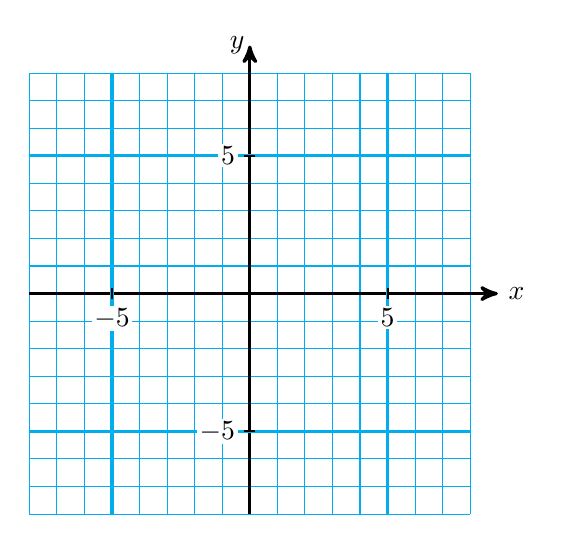
\begin{tikzpicture} [scale=.35]
\draw[cyan] (-8,-8) grid (8,8);
\draw[black,very thick, ->, >=stealth'] (-8,0)--(9,0) node[right]{$x$};
\draw[black,very thick, ->, >=stealth'] (0,-8)--(0,9) node[left, xshift=2]{$y$};
\foreach \x  in  {-5, 5} {
 \draw[cyan, very thick] (\x,-8) --++(0,16);
 \draw[cyan, very thick] (-8,\x) --++(16,0);
 \draw[black, thick] (\x,.2) --++(0,-.4) node[below, yshift=-2, fill=white, inner sep=1]   {$\x$};
 \draw[black,thick] (.2,\x) --++(-.4,0) node[left, xshift=-2, fill=white, inner sep=1]   {$\x$};
}
\end{tikzpicture}
\newline

hp-4-5-17ans

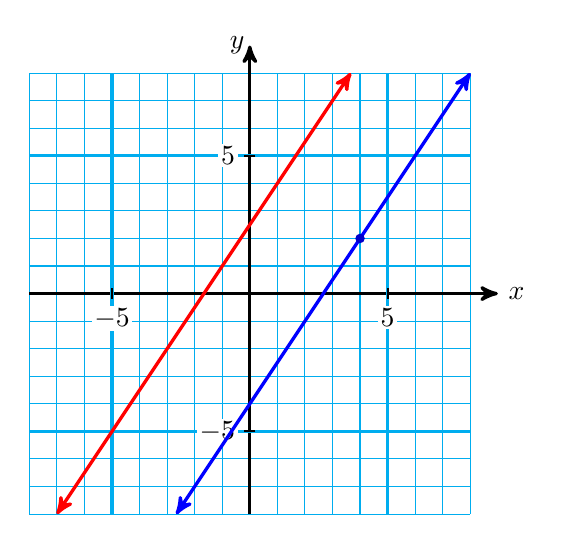
\begin{tikzpicture} [scale=.35]
\draw[cyan] (-8,-8) grid (8,8);
\draw[black,very thick, ->, >=stealth'] (-8,0)--(9,0) node[right]{$x$};
\draw[black,very thick, ->, >=stealth'] (0,-8)--(0,9) node[left, xshift=2]{$y$};
\foreach \x  in  {-5, 5} {
 \draw[cyan, very thick] (\x,-8) --++(0,16);
 \draw[cyan, very thick] (-8,\x) --++(16,0);
 \draw[black, thick] (\x,.2) --++(0,-.4) node[below, yshift=-2, fill=white, inner sep=1]   {$\x$};
 \draw[black,thick] (.2,\x) --++(-.4,0) node[left, xshift=-2, fill=white, inner sep=1]   {$\x$};
}
\draw[red, very thick,<->, >=stealth'] (11/3,8)--(-7,-8);
\draw[blue, very thick,<->, >=stealth'] (8,8)--(-8/3,-8);
\filldraw[blue!80!black] (4,2) circle (1.5mm);
\end{tikzpicture}
\newline


\section{Chap 4 review}

cr4-43ans

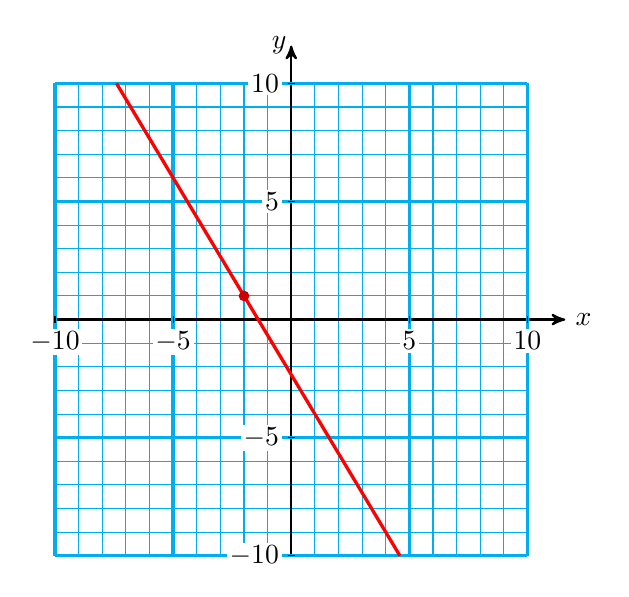
\begin{tikzpicture} [scale=.3]
\coordinate (O) at (0,0);
\draw[cyan] (-10,-10) grid (10,10);
\draw[black,thick, ->, >=stealth'] (-10,0)--(11.6,0) node[right]{$x$};
\draw[black,thick, ->, >=stealth'] (0,-10)--(0,11.6) node[left, xshift=2]{$y$};
\foreach \x in  {-5, 5, -10, 10} {
 \draw[cyan, very thick] (\x,-10) --++(0,20);
 \draw[cyan, very thick] (-10,\x) --++(20,0);
 \draw[black] (\x,.15) --++(0,-.3)  node[below, yshift=-2, fill=white, inner sep=1]   {$\x$};
 \draw[black] (.15,\x) --++(-.3,0)  node[left, xshift=-2, fill=white, inner sep=1]   {$\x$};
}
\draw[red,very thick] (23/5,-10)--(-37/5,10);
\filldraw[red!80!black] (-2,1) circle (2mm);
\end{tikzpicture}
\newline



\section{Other stuff}

10 by 10 grid: hp-2-3-12

8 by 8 grid: hp-4-5-17

\end{document}
